\documentclass[a4paper,12pt]{article}

\usepackage[utf8]{inputenc}
\usepackage[T1]{polski}
\usepackage{helvet}
\usepackage{graphicx}
\usepackage{color}
\usepackage{xcolor}
\usepackage{geometry}
\usepackage{caption}
\usepackage{makeidx}
\usepackage{multirow}
\usepackage{wrapfig}
\usepackage{listings}


\geometry{hmargin={2cm, 2cm}, height=10.0in}
\DeclareCaptionFont{white}{\color{white}}
\DeclareCaptionFormat{listing}{\colorbox{gray}{\parbox{\textwidth}{#1#2#3}}}
\captionsetup[lstlisting]{format=listing,labelfont=white,textfont=white}
\lstset{ %
language=Octave,                % choose the language of the code
basicstyle=\footnotesize,       % the size of the fonts that are used for the code
numbers=left,                   % where to put the line-numbers
numberstyle=\footnotesize,      % the size of the fonts that are used for the line-numbers
stepnumber=1,                   % the step between two line-numbers. If it's 1 each line 
                                % will be numbered
numbersep=5pt,                  % how far the line-numbers are from the code
backgroundcolor=\color{white},  % choose the background color. You must add \usepackage{color}
showspaces=false,               % show spaces adding particular underscores
showstringspaces=false,         % underline spaces within strings
showtabs=false,                 % show tabs within strings adding particular underscores
frame=single,	                % adds a frame around the code
tabsize=2,	                % sets default tabsize to 2 spaces
%captionpos=b,                   % sets the caption-position to bottom
breaklines=true,                % sets automatic line breaking
breakatwhitespace=false,        % sets if automatic breaks should only happen at whitespace
title=\lstname,                 % show the filename of files included with \lstinputlisting;
                                % also try caption instead of title
escapeinside={\%*}{*)},         % if you want to add a comment within your code
morekeywords={*,...}            % if you want to add more keywords to the set
}

\lstloadlanguages{ Ruby }


\makeindex

\begin{document}

% =====  STRONA TYTULOWA PRACY INŻYNIERSKIEJ ====
% ostatnia modyfikacja: 2009/07/01, K. Malarz

\thispagestyle{empty}

%% ------------------------ NAGLOWEK STRONY ---------------------------------
\begin{figure}
\vspace{-13cm}
\hspace{-4cm}

\includegraphics[height=29.3cm]{grafika/agh_nzw_a_pl_1w_wbr_cmyk.pdf}\\
\vspace{-13.9cm}
\end{figure}
\rule{26mm}{0pt}
{\large\textsf{Wydział Fizyki i Informatyki Stosowanej}}\\
\rule{\textwidth}{3pt}\\
\rule[2ex]
{\textwidth}{1pt}\\
\vspace{7ex}
\begin{center}
{\bf\LARGE\textsf{Analiza i przetwarzanie obrazów}}\\
\vspace{13ex}
{\bf\huge\textsf{Ćwiczenie 1}}\\
\vspace{3ex}
{\sf \small } {\bf\small\textsf{Krystian Wojtas}}\\
\vspace{14ex}
%% ------------------------ OPIEKUN PRACY ------------------------------------
{\sf \Large } {\bf\Large\textsf{}}\\
\vspace{22ex}
\textsf{\bf\large\textsf{Kraków, październik 2011}}
\end{center}
%% =====  STRONA TYTUŁOWA PRACY INŻYNIERSKIEJ  ====


\newpage
\section{Wstęp}
Celem ćwiczeń było kilka podstawowych przekształceń kolorystyki obrazu. Wykorzystany został język Ruby i jego framework RMagic, który binduje funkcje biblioteczne z pakietu ImageMagick.

\subsection{Terminy}
\begin{description}
  \item[Piksel] \hfill \\
  Jest to najmniejszy element obrazu cechujący się nadanym mu kolorem. Kolor w przestrzeni barw RGB reprezentuje ważona mieszanka z kanałów podstawowych kolejno czerwonego, zielonego i niebieskiego.
\end{description}

\subsection{Obraz przetwarzany}
\begin{figure}[h!]
   \centering
   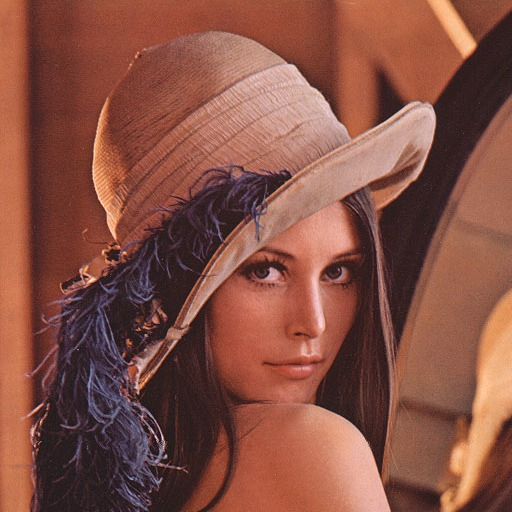
\includegraphics[width=15cm]{../../lena.jpg}
   \caption{Obraz poddawany obróbce}
\end{figure}


\newpage
\section{Negatyw}
Efekt negatywu uzyskujemy poprzez odwrócenia barw.
$$p(r, g, b) = p(255-r, 255-g, 255-b)$$
\begin{figure}[h!]
   \centering
   \includegraphics[width=15cm]{../out/negate.jpg}
   \caption{Negatyw}
\end{figure}


\newpage

\begin{figure}
\begin{minipage}[t]{7.5cm}
\begin{center}
\includegraphics[width=7.5cm,clip]{../out/negate.jpg}
\caption{Implementacja}
\end{center}
\end{minipage}
\hfill
\begin{minipage}[t]{7.5cm}
\begin{center}
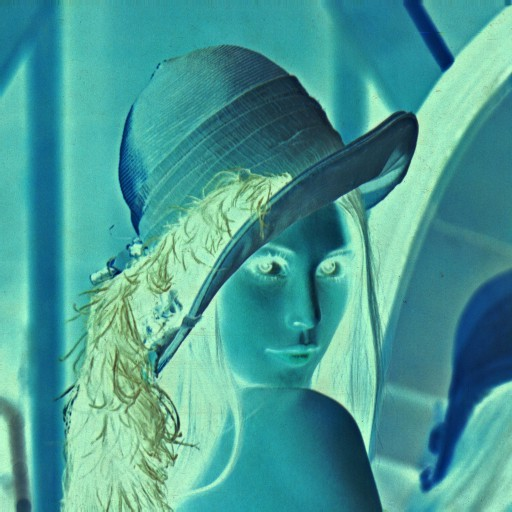
\includegraphics[width=7.5cm,clip]{grafika/negate_magick.jpg}
\caption{Funkcja biblioteczna}
\end{center}
\end{minipage}
\end{figure} 

Widać, że osiągnięte efekty są bardzo podobne, jeśli nie identyczne.

\lstinputlisting[caption=Implementacja efektu negatywu]{listingi/negate.rb}
\lstinputlisting[caption=Obciecie wartosci wykraczajacych poza zakres]{listingi/tools_cut.rb}


\newpage
\section{Odcienie szarości 1}
Obraz w odcieniach szarości uzyskujemy uśredniając wartości kanałów w pixelach.
$$sr_{p(r,g,b)} = (r + g + b) / 3$$
$$p(r, g, b) = p( sr_{p(r,g,b)}, sr_{p(r,g,b)}, sr_{p(r,g,b)})$$
\begin{figure}[h!]
   \centering
   \includegraphics[width=15cm]{../out/grayscale1.jpg}
   \caption{Odcienie szarości 1}
\end{figure}
\lstinputlisting[caption=Implementacja odcieni szarosci 1. rodzaju]{listingi/grayscale1.rb}


\newpage
\section{Odcienie szarości 2}
Obraz bardziej naturalny dla ludzkiego oka uzyskuje się przez uśrednienie barw z różnymi wagami.
$$sr_{p(r,g,b)} = 0.3r + 0.59g + 0.11b$$
$$p(r, g, b) = p( sr_{p(r,g,b)}, sr_{p(r,g,b)}, sr_{p(r,g,b)})$$
\begin{figure}[h!]
   \centering
   \includegraphics[width=15cm]{../out/grayscale2.jpg}
   \caption{Odcienie szarości 2}
\end{figure}
\lstinputlisting[caption=Implementacja odcieni szarosci 2. rodzaju]{listingi/grayscale2.rb}


\newpage
\section{Histogram}
Histogram rozpina zapisany zakres barw w obrazie na całą możliwą przestrzeń. W tym celu należy najpierw znaleźć na obrazie wartości minimalne i maksymalne dla każdej z barwy. Następnie znormalizować.
$$p(x, y) = (p(x, y) - min) / (max - min) * 255$$
\begin{figure}[h!]
   \centering
   \includegraphics[width=15cm]{../out/histogram.jpg}
   \caption{Histogram}
\end{figure}

\begin{table}[h!]
\centering
\begin{tabular}{|r|c|c|}
  \hline 
  Red & 13878 & 65535\\
  \hline
  Green & 0 & 61423 \\
  \hline
  Blue & 6939 & 57825 \\
  \hline
\end{tabular} 
\caption{Zakresy poszczególnych barw obrazu wzorcowego}
\end{table}


\newpage

\begin{figure}
\begin{minipage}[t]{5cm}
\begin{center}
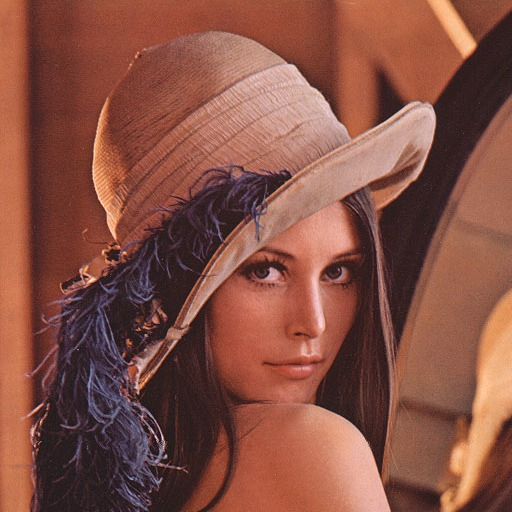
\includegraphics[width=5cm,clip]{../../lena.jpg}
\caption{Wzorzec}
\end{center}
\end{minipage}
\hfill
\begin{minipage}[t]{5cm}
\begin{center}
\includegraphics[width=5cm,clip]{../out/histogram.jpg}
\caption{Implementacja}
\end{center}
\end{minipage}
\hfill
\begin{minipage}[t]{5cm}
\begin{center}
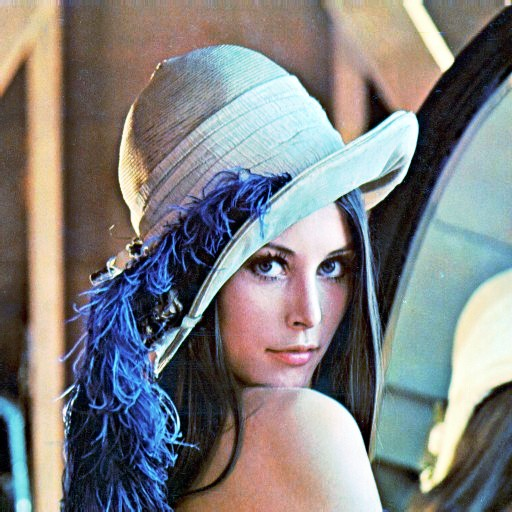
\includegraphics[width=5cm,clip]{grafika/histogram_magick.jpg}
\caption{Funkcja biblioteczna}
\end{center}
\end{minipage}
\end{figure} 

Każdy kanał barwy normalizowałem oddzielnie. Dzięki temu obraz wydaje się "lepszy" od wzorca, a przy tym nie odbiega kolorystyką tak jak wynik działania funkcji bibliotecznej.

\lstinputlisting[caption=Poszukiwanie ekstremow zadanego kanalu]{listingi/ekstrema.rb}
\lstinputlisting[caption=Implementacja efektu normalizacji barw]{listingi/histogram.rb}

\newpage
\subsection{Histogram skali szarości}

\begin{figure}[ht!]
\begin{minipage}[t]{7.5cm}
\begin{center}
\includegraphics[width=7.5cm,clip]{../out/grayscale1.jpg}
\caption{Odcienie szarości 1}
\end{center}
\end{minipage}
\hfill
\begin{minipage}[t]{7.5cm}
\begin{center}
\includegraphics[width=7.5cm,clip]{../out/grayscale1_histogram.jpg}
\caption{Hisotgram w szarości 1}
\end{center}
\end{minipage}
\end{figure} 

\begin{figure}[ht!]
\begin{minipage}[t]{7.5cm}
\begin{center}
\includegraphics[width=7.5cm,clip]{../out/grayscale2.jpg}
\caption{Odcienie szarości 2}
\end{center}
\end{minipage}
\hfill
\begin{minipage}[t]{7.5cm}
\begin{center}
\includegraphics[width=7.5cm,clip]{../out/grayscale2_histogram.jpg}
\caption{Hisotgram w szarości 2}
\end{center}
\end{minipage}
\end{figure} 

\lstinputlisting[caption=Implementacja efektu normalizacji barw dla odcieni szarosci]{listingi/histogram_grayscale.rb}

\end{document}
